\titre{}
\theme{Calcul différentiel}
\auteur{Nathan Scheinmann}
\niveau{3M}
\source{}
\type{serie}
\piments{}
\pts{}
\annee{2526}

\contenu{
	\tcblower
	On donne le graphe d'une fonction $f$. Esquisser le graphe de $f'$.
% Écrivez l'énoncé de l'exercice ici
\begin{tasks}(2)
	\task

	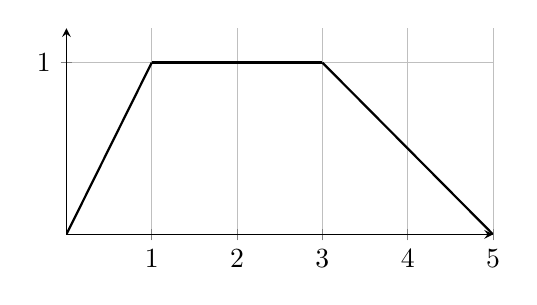
\begin{tikzpicture}
\begin{axis}[
  width=7cm,height=4.2cm,
  axis lines=middle, grid=both,
  xmin=0, xmax=5, ymin=0, ymax=1.2,
  xtick={0,1,2,3,4,5}, ytick={0,1},
]
  \addplot[thick] coordinates {(0,0) (1,1)};
  \addplot[thick] coordinates {(1,1) (3,1)};
  \addplot[thick] coordinates {(3,1) (5,0)};
\end{axis}
\end{tikzpicture}
\task 


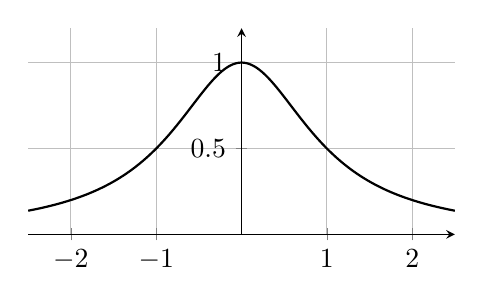
\begin{tikzpicture}
\begin{axis}[
  width=7cm,height=4.2cm,
  axis lines=middle, grid=both,
  xmin=-2.5, xmax=2.5, ymin=0, ymax=1.2,
  xtick={-2,-1,0,1,2}, ytick={0,0.5,1},
]
  \addplot[domain=-2.5:2.5, samples=300, thick]
    {1/(1 + x^2)};
\end{axis}
\end{tikzpicture}

\task 


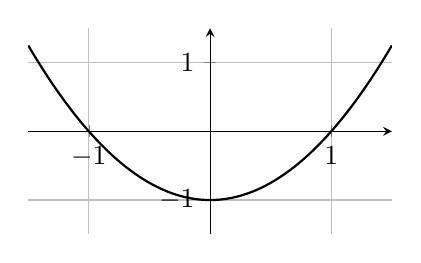
\begin{tikzpicture}
\begin{axis}[
  width=6.2cm,height=4.2cm,
  axis lines=middle, grid=both,
  xmin=-1.5, xmax=1.5, ymin=-1.5, ymax=1.5,
  xtick={-1,0,1}, ytick={-1,0,1},
]
  \addplot[domain=-1.5:1.5, samples=200, thick]
    {x^2 - 1};
\end{axis}
\end{tikzpicture}


\task 


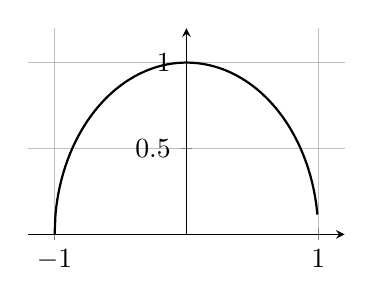
\begin{tikzpicture}
\begin{axis}[
  width=5.6cm,height=4.2cm,
  axis lines=middle, grid=both,
  xmin=-1.2, xmax=1.2, ymin=0, ymax=1.2,
  xtick={-1,0,1}, ytick={0,0.5,1},
]
  \addplot[domain=-1:1, samples=300, thick]
    {sqrt(1 - x^2)};
\end{axis}
\end{tikzpicture}
\end{tasks}
}
\correction{
% Écrivez la correction ici

}
